\begin{comment}
\section{JavaScript e a Programação Assíncrona}
A linguagem \textit{JavaScript} teve a sua origem no \textit{browser} \textit{Netscape Navigator} como uma forma de adicionar programas a páginas web.~\cite{elojs} Hoje em dia é usado por grande parte dos \textit{browsers} e tornou possível as aplicações web onde o utilizador pode interagir sem precisar de realizar \textit{refresh} ao fim de cada ação.
Contudo o \textit{Javascript} é bastante liberal no que permite o programador escrever, facilitando a aprendizagem para novos programadores mas tornando a tarefa de resolver e encontrar problemas bem mais difícil visto não apontar aonde estão esses problemas. Ainda assim esta flexibilidade permite uma quantidade de técnicas que não são possíveis em linguagens mais rígidas e que permitem ultrapassar algumas falhas do \textit{Javascript}.~\cite{elojs} 

\subsection{Programação Assíncrona}
Muitos programas em \textit{JavaScript} precisam de por exemplo obter dados através da rede ou a partir do disco. Estes casos são muito mais lentos do que obter os dados a partir de memória para posterior processamento pelo processador. Na realização de tais pedidos o programa em \textit{Javascript} perderia o acesso ao processador, passando este acesso para outro programa que esteja a correr. Só depois de receber o sinal de que o pedido foi efetuado e de ter de novo acesso ao processador é que o programa voltaria a continuar o seu trabalho.

Por forma a evitar perder o acesso do processador em tais casos, e assim realizar trabalho enquanto se espera pela resposta do pedido, o \textit{Javascript} segue um modelo assíncrono. O modelo assíncrono permite que aconteçam várias coisas ao mesmo tempo; quando começa um pedido o programa continua a correr; quando o pedido termina, o programa é informado e tem acesso ao resultado.~\cite{elojs} Para além de não se perder imediatamente o acesso ao processor, o uso de programação assíncrona permite receber e enviar dados de e para múltiplos dispositivos ao mesmo tempo sem complicar a gestão de \textit{threads} e a sincronização necessária em tais casos. Ao usar um modelo assíncrono a expressão de programas que não seguem um modelo de controlo linear é mais fácil enquanto que torna mais difícil aqueles que o seguem.~\cite{elojs}

\subsubsection{\textit{Callbacks}}
Uma abordagem de programação assíncrona é a adição de um argumento extra, uma função \textit{callback}, nas funções que realizam pedidos lentos.~\cite{elojs} Quando o pedido concluir a função \textit{callback} será chamada tendo como argumento o resultado do pedido. Com o uso de callbacks o nível de indentação aumenta com cada pedido assíncrono o que em alguns casos pode tornar o código um pouco difícil de compreender, principalmente nos casos com múltiplos pedidos assíncronos seguidos que têm de ser sequenciais. Para além disso, qualquer função que chame uma função assíncrona tem de ser ela própria assíncrona. Não é recomendado a reestruturação de grandes quantidades de código através de \textit{callbacks} visto ser mais propenso a erros do que retornar apenas um valor.

\begin{lstlisting}[language=JavaScript, caption=Exemplo de uma \textit{Callback}]
    almocar("comida", function(dentes%*\_*)sujos)%*\{*)
        dentes%*\_*)limpos = lavar%*\_*)dentes(dentes%*\_*)sujos)
    %*\}*))
\end{lstlisting}

\subsubsection{Promessas}
Uma outra abordagem, em vez de passar uma função a ser chamada no futuro, é devolver um objeto que represente este evento futuro, uma promessa. Ou seja, uma promessa é um pedido assíncrono que pode ser concluído no futuro e produzir um valor, tendo a capacidade de notificar qualquer interessado quando o valor estiver disponível.\cite{elojs} O resultado de uma promessa tanto pode já estar pronto ou estar apenas daqui a algum tempo. A principal vantagem das promessas é que simplificam o uso de funções assíncronas visto que não é necessário passar uma função \textit{callback}. Como tal estas funções são similares às restantes mas com uma pequena diferença, o resultado da função pode ainda não estar disponível. 

\begin{lstlisting}[language=JavaScript, caption=Exemplo de uma Promessa]
    almocar("comida")
        .then(dentes%*\_*)sujos =%*$>$*) dentes%*\_*)limpos = lavar%*\_*)dentes(dentes%*\_*)sujos))
\end{lstlisting}

\subsubsection{Exceções}
Durante a execução de um pedido assíncrono podem ocorrer exceções seja por um erro ou porque por exemplo ocorreu um \textit{time out} do pedido, este último acontece essencialmente quando se realiza pedidos através da rede. Estas exceções precisam de ser tratadas por forma a que o programa que estámos a desenvolver não ``expluda'' deixando de funcionar. Esta tratamento não é simples de se realizar quando se usa \textit{callbacks} enquanto que no caso das promessas basta o uso de um \textit{catch}. No caso das \textit{callbacks} o pedido assíncrono teria de devolver dois valores em vez de um, o primeiro com o erro em caso de insucesso e o segundo com o resultado em caso de sucesso o que obrigaria a função \textit{callback} a verificar se não recebeu uma exceção.

\begin{lstlisting}[language=JavaScript, caption=Exemplo de uma \textit{Callback} com captura de exceções]
    almocar("comida", function(erro, dentes%*\_*)sujos)%*\{*)
        if(!erro)%*\{*)
            dentes%*\_*)limpos = lavar%*\_*)dentes(dentes%*\_*)sujos)
        %*\}*)else%*\{*)
            console.log("Falta pasta de dentes")
        %*\}*)
    %*\}*))
\end{lstlisting}

\begin{lstlisting}[language=JavaScript, caption=Exemplo de uma Promessa com captura das exceções]
    almocar("comida")
        .then(dentes%*\_*)sujos =%*$>$*) dentes%*\_*)limpos = lavar%*\_*)dentes(dentes%*\_*)sujos))
        .catch(erro =%*$>$*) console.log("Falta pasta de dentes"))
\end{lstlisting}

\subsubsection{Funções \textit{async}}
Dentro de funções \textit{async} é possível escrever código pseudo-síncrono por forma a descrever código assíncrono com recurso ao \textit{await} que espera pela conclusão de uma promessa antes de avançar com a execução do resto da função, ficando o código com um aspeto semelhante ao síncrono. As funções \textit{async} retornam implicitamente uma promessa e enquanto estão à espera duma promessa (\textit{await}) ficam congeladas. Serão resumidas mais tarde quando a promessa estiver concluída.

\begin{lstlisting}[language=JavaScript, caption=Exemplo de uma função \textit{async}]
    async function almoco()%*\{*)
        try%*\{*)
            dentes%*\_*)sujos = await almocar("comida")
            dentes%*\_*)limpos = lavar%*\_*)dentes(dentes%*\_*)sujos)
        %*\}*)catch(erro)%*\{*)
            console.log("Falta pasta de dentes")
        %*\}*)
        return "Almocei!"
    %*\}*)
\end{lstlisting}

\section{Node.js}
\textit{Node.js} é um ambiente de execução que permite usar \textit{JavaScript} fora do contexto de um \textit{browser} permitindo construir desde ferramentas de linha de comandos até servidores \acrshort{http}. Foi originalmente desenhado de forma a ter o papel de nodo numa rede. O \textit{JavaScript} não tem embutido a capacidade de entrada e saída de dados sendo suprimida esta necessidade com o uso do \textit{Node.js}.

Quando instalado num sistema, o \textit{Node.js} permite executar ficheiros \textit{JavaScript} através do comando \texttt{node}. Se este comando for executado sem indicar um ficheiro apresenta uma consola interativa onde se pode introduzir código \textit{JavaScript}, executá-lo e obter o resultado.

Através do \acrshort{npm}, mais precisamente do comando \texttt{npm}, é possível instalar, no nosso projeto pessoal, os módulos \textit{JavaScript} disponíveis no repositório \textit{online}. Caso exista um ficheiro \textit{package.json} no projeto é mantido neste os módulos já instalados e as suas versões bem como meta informação do projeto.

Em \textit{Node.js} estão disponíveis os \textit{bindings} globais \texttt{process} e \texttt{console} que permitem inspecionar e manipular o programa atual. Para além destes, também estão diponíveis os \textit{bindings} padrão do \textit{JavaScript} exceto aqueles relacionados com funcionalidades do \textit{browser}, como o \texttt{document}.

O \textit{Node.js} tem algums módulos embutidos, entre os quais o módulo \texttt{fs} (\textit{file system}) que exporta funções que permitem trabalhar com ficheiros e directorias. Tem também o módulo \texttt{http} que exporta funções que permitem correr servidores \acrshort{http} ou fazer pedidos \acrshort{http}.

Todo o input e output no \textit{Node.js} é realizado de forma assíncrona a menos que se use uma variante síncrona de uma determinada função.~\cite{elojs}
\end{comment}

\section{Estado da Arte do \acrshort{clav}}

Quando esta dissertação teve início o projeto \acrshort{clav} já tinha cerca de 2 anos de desenvolvimento. Assim nesta secção será apresentado o estado da arte do \acrshort{clav} quando esta dissertação iniciou aprofundando principalmente os pontos mais importantes sobre o tema desta dissertação.

\subsection{Estrutura}
O \acrshort{clav} está dividido em duas partes:
\begin{itemize}
    \item interface (\textit{front-end}) presente em \url{http://clav.dglab.gov.pt}
    \item \acrshort{api} de dados (\textit{back-end} que inclui também duas bases de dados, \textit{GraphDB} e \textit{MongoDB}) presente em \url{http://clav-api.dglab.gov.pt}.
\end{itemize}

Cada parte encontra-se numa máquina diferente.

Através da figura~\ref{fig:clav_struct} é possível ver o possível fluxo tanto de um utilizador a aceder à interface como a de um utilizador a aceder diretamente à \acrshort{api} de dados. No primeiro caso, quando um utilizador acede o servidor da interface do \acrshort{clav} é descarregado para o lado do utilizador o ficheiro \acrshort{html} (\textit{index}) e os vários ficheiros \textit{JavaScript}, \acrshort{css} e \textit{assets} (como imagens, \acrshort{pdf}s, etc) quando necessários. O servidor da interface é nada mais que um servidor \textit{web} com recurso ao \textit{Nginx} que hospeda estes ficheiros, os quais representam a interface construída com o \textit{Vue} e o \textit{Vuetify}. Como tal o código apresenta-se todo do lado do utilizador e os pedidos à \acrshort{api} serão feitos do computador do utilizador para o servidor da \acrshort{api} de dados e não do servidor da interface para o servidor da \acrshort{api} de dados. Ou seja, o fluxo de cada um desses pedidos será igual ao fluxo no caso em que se acede diretamente a \acrshort{api} sem uso de qualquer interface.

\begin{figure}[H]
    \begin{center}
        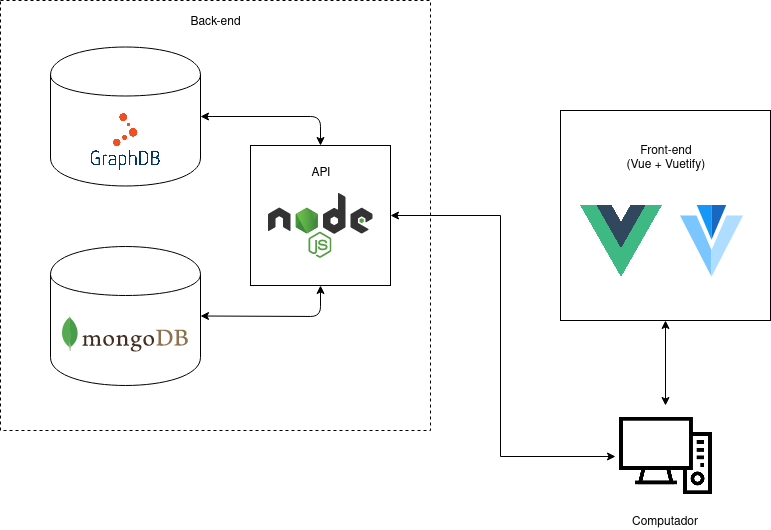
\includegraphics[width=0.7\textwidth]{img/clav_struct.png}
    \end{center}
    \caption{Estrutura do \acrshort{clav} incluíndo a interação de um utilizador com a mesma}
    \label{fig:clav_struct}
\end{figure}

\subsection{Formas de autenticação}
A \acrshort{api} de dados e a interface estavam inicialmente ``juntas'' (aplicação monolítica) onde as rotas eram protegidas contudo, com a separação da aplicação em duas partes, ambas partes deixaram de estar protegidas. Devido à plataforma já ter estado protegida esta já possui duas formas de autenticação, através de chaves \acrshort{api} ou através de utilizadores registados. Ou seja, tanto o registo de utilizadores e de chaves API já se encontra implementado bem como o \textit{login} de utilizadores.

As chaves \acrshort{api} existem por forma a dar acesso a certas rotas da \acrshort{api} a aplicações que interajam com a mesma (por exemplo sistemas de informação) sem a necessidade de interação humana.

Já os utilizadores possuem múltiplos níveis de acesso sendo que consoante o seu nível podem ou não aceder a uma rota da interface ou da \acrshort{api}. Os utilizadores podem autenticarem-se através de \textit{email} e \textit{password} ou com recurso ao \acrfull{cc} através do Autenticação.gov.

A hierarquia dos níveis de acesso, do nível que permite menor para o maior acesso é a seguinte:
\begin{itemize}
    \item Nível 0: Chaves API
    \item Nível 1: Representante Entidade
    \item Nível 2: Utilizador Simples
    \item Nível 3: Utilizador Avançado
    \item Nível 3.5: Utilizador Validador (AD)
    \item Nível 4: Utilizador Validador
    \item Nível 5: Utilizador Decisor
    \item Nível 6: Administrador de Perfil Funcional
    \item Nível 7: Administrador de Perfil Tecnológico
\end{itemize}

As chaves \acrshort{api} poderão aceder a algumas rotas com método \texttt{GET}.
Já os utilizadores poderão realizar todos os pedidos que as chaves \acrshort{api} podem realizar mas quanto maior o seu nível de acesso mais rotas poderão aceder.

A proteção da \acrshort{api} terá de ter esta hierarquia em conta.

\subsubsection{Registo}

Para o registo de uma chave \acrshort{api} é necessário providenciar um nome, um email e a entidade a que pertence.

Um utilizador podia inicialmente se registar através de \texttt{email + password} ou através do Autenticação.gov. No primeiro caso, ao se registar necessita obviamente de indicar o seu email, a \textit{password}, o seu nome, a entidade a que pertence e o nível de acesso que pretende. Já no caso do Autenticação.gov para o registo do utilizador é necessário todos os campos anteriores exceto a \textit{password} (pode ser depois definida), sendo também necessário o campo \acrfull{nic} do utilizador. Caso o registo seja efetuado com recurso à interface do Autenticação.gov apenas será necessário indicar o email, a entidade a que pertence e o nível de acesso que pretende visto que os restantes campos são fornecidos pela Autenticação.gov quando o utilizador se autentica e autoriza nesta a partilha dessa informação com a plataforma do \acrshort{clav}.
A \textit{password} é armazenada não na sua forma literal mas sim a sua \textit{hash} ao aplicar a função criptográfica \texttt{bcript}.

\subsubsection{A melhorar}

As duas formas de autenticação necessitam de melhorias. Uma delas é a possibilidade de o \acrshort{jwt} do utilizador puder ser enviado no \texttt{body} algo que nem todos os métodos \acrshort{http} permitem bem como o \textit{Swagger} que iremos falar mais à frente não suporta a documentação desta forma de autenticação com \acrshort{jwt}'s. Logo deve ser removido este tipo de autenticação.

\subsection{Lista Consolidada}

\subsection{Tabelas de Seleção}

\subsection{Cache e Fecho Transitivo}

\section{\acrshort{rest}}
\cite{restws}

%\section{express}
%\cite{wdmongo}
%procurar "semelhantes" para cada um

%\section{passport}
%procurar "semelhantes" para cada um

\section{jsonwebtoken}
%conceito JWT
%procurar "semelhantes" para cada um

%\section{passport-jwt}
%procurar "semelhantes" para cada um

\section{CORS}
%falar da package e do conceito CORS
%procurar "semelhantes" para cada um

%\section{axios}
%procurar "semelhantes" para cada um

\section{HTTP Status}

\section{Headers do HTTP}

\section{Autenticação.gov}
\cite{agov}

%\section{exceljs}
%procurar "semelhantes" para cada um

\section{MongoDB}
\cite{wdmongo}

%\section{mongoose}
%procurar "semelhantes" para cada um

\section{Web Semântica}
\cite{lsparql}

\subsection{RDF}
\cite{lsparql}

\subsection{SPARQL}
\cite{lsparql}

%se calhar referir algumas packages de ligação ao sparql em vez de usar o que criei

\section{GraphDB}
%procurar "semelhantes" para cada um (Neo4j)

\section{Swagger}
%procurar "semelhantes" para cada um

\section{Swagger-UI}

%\section{yaml-include}
%procurar "semelhantes" para cada um

%\section{swagger-ui-express}
%procurar "semelhantes" para cada um

%\section{js-yaml}
%procurar "semelhantes" para cada um

\section{Nginx}
\cite{nginxcook}
%procurar "semelhantes" para cada um

\section{Ontologia}
\cite{bontology}
%conceito

\section{Docker}
\cite{udocker}
%procurar "semelhantes" para cada um

\section{Docker Compose}
\cite{udocker}
%procurar "semelhantes" para cada um
